%%%%%%%%%%%%%%%%%%%%%%%%%%%%%%%%%%%%%%%%%%%%%%%%%%%%%%%%%%%%%%%%%%%%
%% appendix1.tex
%% UNL thesis document file
%%
%% Chapter with example of appendix with a short dummy text
%%%%%%%%%%%%%%%%%%%%%%%%%%%%%%%%%%%%%%%%%%%%%%%%%%%%%%%%%%%%%%%%%%%%
\chapter{Código da aplicação}
\label{cha:codigo_da_aplicacao}

\begin{figure}[hbtp]
	\centering
	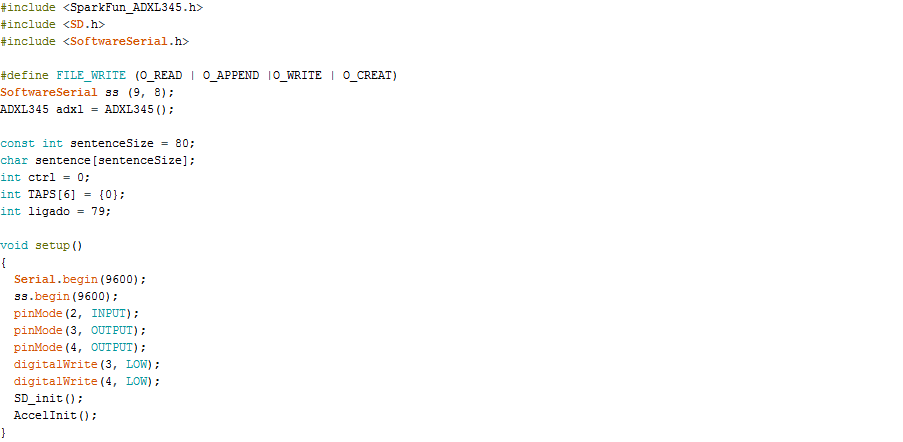
\includegraphics[width=14cm]{ard1}
	\caption{Zona de inicialização e função setup}
	\label{fig:ard1}
\end{figure}

\begin{figure}[hbtp]
	\centering
	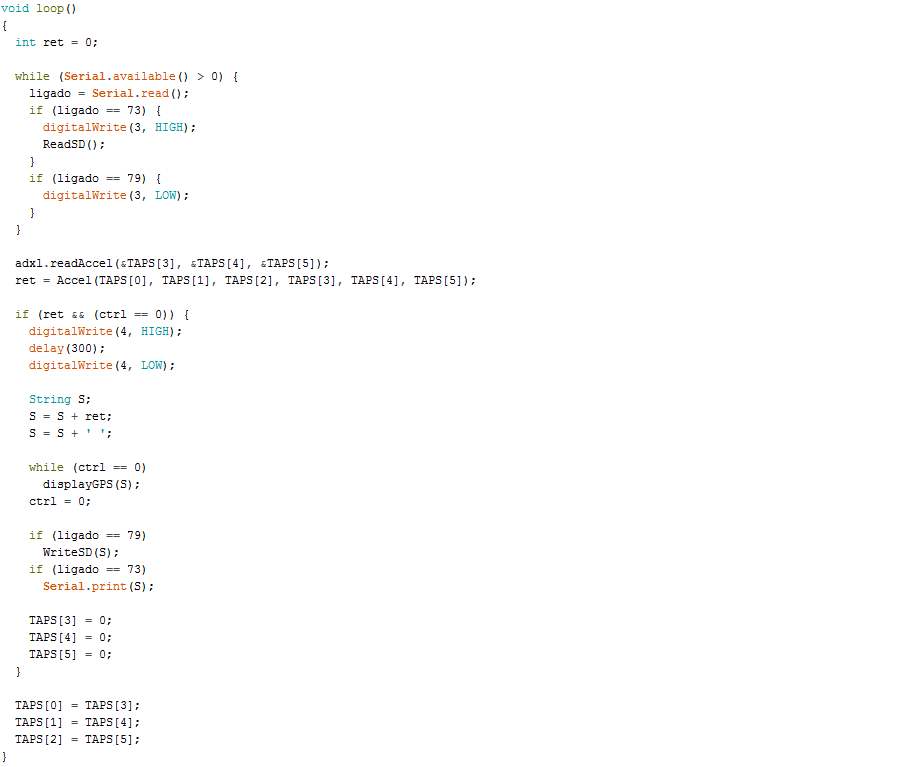
\includegraphics[width=14cm]{ard2}
	\caption{Função loop}
	\label{fig:ard2}
\end{figure}

\begin{figure}[hbtp]
	\centering
	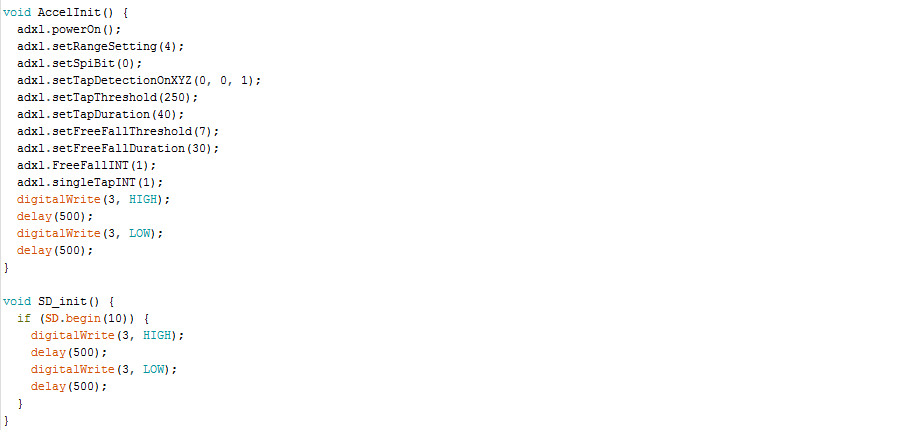
\includegraphics[width=14cm]{ard3}
	\caption{Funções accelInit e SD\textunderscore init}
	\label{fig:ard3}
\end{figure}

\begin{figure}[hbtp]
	\centering
	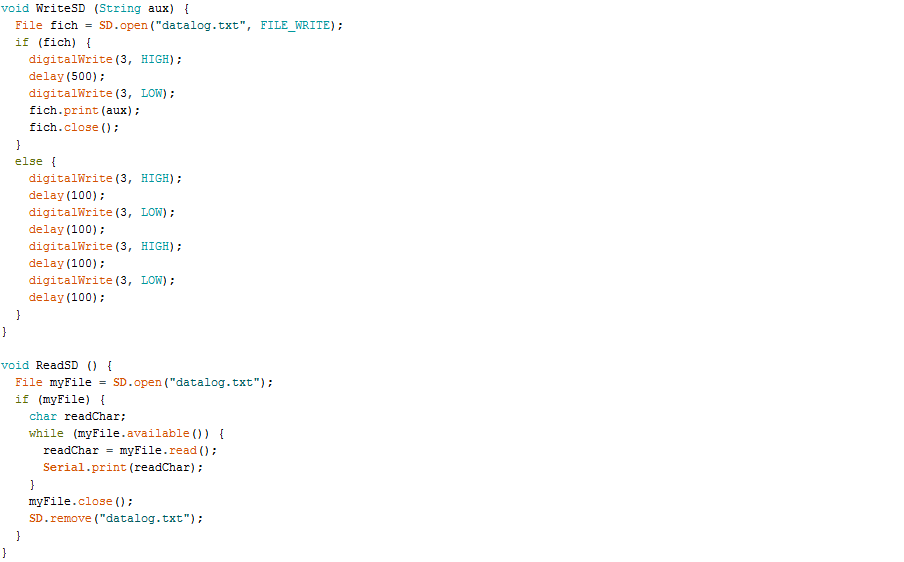
\includegraphics[width=14cm]{ard4}
	\caption{Funções WriteSD e ReadSD}
	\label{fig:ard4}
\end{figure}

\begin{figure}[hbtp]
	\centering
	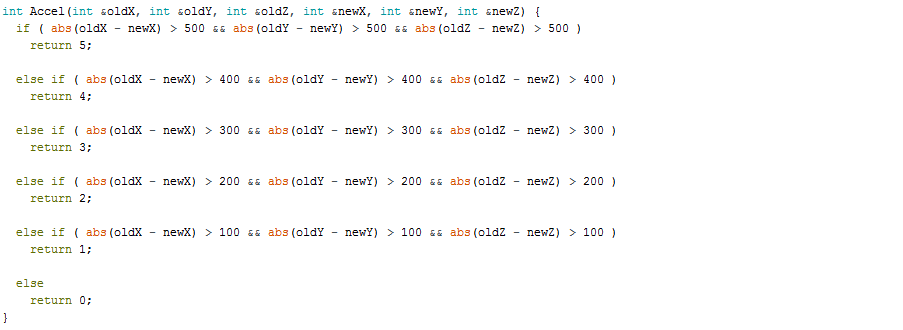
\includegraphics[width=14cm]{ard5}
	\caption{Função Accel}
	\label{fig:ard5}
\end{figure}

\begin{figure}[hbtp]
	\centering
	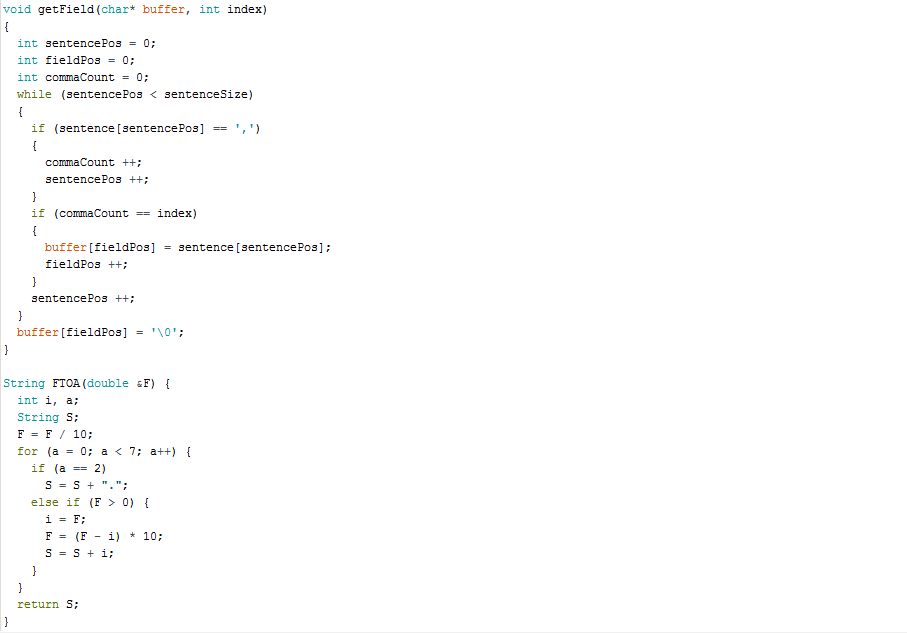
\includegraphics[width=14cm]{ard6}
	\caption{Funções getField e FTOA}
	\label{fig:ard6}
\end{figure}